%%%%%%%%%%%%%%%%%%%%%%%%%%%%%%%%%%%%%%%%%%%%%%%%%%%%%%%%%%%%%%%%%%%%%
%%                                                                 %%
%% Please do not use \input{...} to include other tex files.       %%
%% Submit your LaTeX manuscript as one .tex document.              %%
%%                                                                 %%
%% All additional figures and files should be attached             %%
%% separately and not embedded in the \TeX\ document itself.       %%
%%                                                                 %%
%%%%%%%%%%%%%%%%%%%%%%%%%%%%%%%%%%%%%%%%%%%%%%%%%%%%%%%%%%%%%%%%%%%%%

%%\documentclass[referee,sn-basic]{sn-jnl}% referee option is meant for double line spacing

%%=======================================================%%
%% to print line numbers in the margin use lineno option %%
%%=======================================================%%

%%\documentclass[lineno,sn-basic]{sn-jnl}% Basic Springer Nature Reference Style/Chemistry Reference Style

%%======================================================%%
%% to compile with pdflatex/xelatex use pdflatex option %%
%%======================================================%%

%%\documentclass[pdflatex,sn-basic]{sn-jnl}% Basic Springer Nature Reference Style/Chemistry Reference Style

%%\documentclass[sn-basic]{sn-jnl}% Basic Springer Nature Reference Style/Chemistry Reference Style
\documentclass[pdflatex,sn-mathphys]{sn-jnl}% Math and Physical Sciences Reference Style
%%\documentclass[sn-aps]{sn-jnl}% American Physical Society (APS) Reference Style
%%\documentclass[sn-vancouver]{sn-jnl}% Vancouver Reference Style
%%\documentclass[sn-apa]{sn-jnl}% APA Reference Style
%%\documentclass[sn-chicago]{sn-jnl}% Chicago-based Humanities Reference Style
%%\documentclass[sn-standardnature]{sn-jnl}% Standard Nature Portfolio Reference Style
%%\documentclass[default]{sn-jnl}% Default
%%\documentclass[default,iicol]{sn-jnl}% Default with double column layout

%%%% Standard Packages
%%<additional latex packages if required can be included here>
%%%%
\usepackage{subfig}
\usepackage{booktabs}
\usepackage{multirow}
\usepackage{graphicx}
%%%%%=============================================================================%%%%
%%%%  Remarks: This template is provided to aid authors with the preparation
%%%%  of original research articles intended for submission to journals published 
%%%%  by Springer Nature. The guidance has been prepared in partnership with 
%%%%  production teams to conform to Springer Nature technical requirements. 
%%%%  Editorial and presentation requirements differ among journal portfolios and 
%%%%  research disciplines. You may find sections in this template are irrelevant 
%%%%  to your work and are empowered to omit any such section if allowed by the 
%%%%  journal you intend to submit to. The submission guidelines and policies 
%%%%  of the journal take precedence. A detailed User Manual is available in the 
%%%%  template package for technical guidance.
%%%%%=============================================================================%%%%

\jyear{2021}%

%% as per the requirement new theorem styles can be included as shown below
\theoremstyle{thmstyleone}%
\newtheorem{theorem}{Theorem}%  meant for continuous numbers
%%\newtheorem{theorem}{Theorem}[section]% meant for sectionwise numbers
%% optional argument [theorem] produces theorem numbering sequence instead of independent numbers for Proposition
\newtheorem{proposition}[theorem]{Proposition}% 
%%\newtheorem{proposition}{Proposition}% to get separate numbers for theorem and proposition etc.

\theoremstyle{thmstyletwo}%
\newtheorem{example}{Example}%
\newtheorem{remark}{Remark}%

\theoremstyle{thmstylethree}%
\newtheorem{definition}{Definition}%

\raggedbottom
%%\unnumbered% uncomment this for unnumbered level heads

\begin{document}

% \title{Quantifying and evaluating paste homogeneity from visual perspective}
% \title{Application of vision object detection to homogenize quantization of paste}
\title[Quantitative method for paste homogeneity]{Quantification of paste homogeneity from vision-based identification method}

%%=============================================================%%
%% Prefix	-> \pfx{Dr}
%% GivenName	-> \fnm{Joergen W.}
%% Particle	-> \spfx{van der} -> surname prefix
%% FamilyName	-> \sur{Ploeg}
%% Suffix	-> \sfx{IV}
%% NatureName	-> \tanm{Poet Laureate} -> Title after name
%% Degrees	-> \dgr{MSc, PhD}
%% \author*[1,2]{\pfx{Dr} \fnm{Joergen W.} \spfx{van der} \sur{Ploeg} \sfx{IV} \tanm{Poet Laureate} 
%%                 \dgr{MSc, PhD}}\email{iauthor@gmail.com}
%%=============================================================%%

\author[1]{\fnm{Xiaorui} \sur{Li}}\email{lixiaorui@xs.ustb.edu.cn}

\author[1]{\fnm{Hezheng} \sur{Wang}}\email{M202111287@xs.ustb.edu.cn}
% \equalcont{These authors contributed equally to this work.}

\author[1]{\fnm{Zhaolin} \sur{Yuan}}\email{18810919727@163.com}
% \equalcont{These authors contributed equally to this work.}

\author*[1,2]{\fnm{Xiaojuan} \sur{Ban}}\email{banxj@ustb.edu.cn}
\affil*[1]{\orgdiv{School of Intelligence Science and Technology}, \orgname{University of Science and Technology Beijing}, \orgaddress{\street{Haidian}, \city{Beijing}, \postcode{10083}, \country{China}}}

\affil[2]{\orgdiv{Institute of Artificial Intelligence
}, \orgname{University of Science and Technology Beijing}, \orgaddress{\street{Haidian}, \city{Beijing}, \postcode{100083}, \country{China}}}


\abstract{
% The mixing process is the core part of cemented paste backfill technology, and  
As a core procedure in cemented paste backfill, mixing tailing and cement adequately can improve the paste transportation performance and the physical strength of backfill body. 
Valid quantification of homogeneity can help managers optimize mixing configurations in real-time and ensure adequate mixing. However, there is no real-time quantitative method for paste homogeneity at present. 
To address the problem of measuring paste homogeneity in real-time, this paper proposes a data-driven and non-contact paste homogeneity measurement pipeline to quantify and evaluate paste homogeneity from visual perspectives. 
First, we designed hardware equipment composed of the CMOS camera and server to capture a real-time image of the tail of a double-shaft mixer. 
Second, the paste homogeneity evaluation is formalized as a semantic image segmentation problem. Paste area and non-homogeneous area based were identified on a computer vision algorithm. This is the first time computer vision has been introduced into the problem. 
Then, the non-homogeneity factor is defined as the proportion of the non-homogeneous area to the pasted area.
Finally, Gaussian process regression (GPR) model was used to predict the probability of non-homogeneity factor under the current blade position condition, and the homogeneous metric was calculated according to the probability of the factor.
The experiments conducted in a real industrial paste backfill station demonstrate that the proposed technique satisfies the requirements in terms of efficiency, accuracy and stability, and the quantified metric is consistent with subjective assessment. }

%%================================%%
%% Sample for structured abstract %%
%%================================%%

% \abstract{\textbf{Purpose:} The abstract serves both as a general introduction to the topic and as a brief, non-technical summary of the main results and their implications. The abstract must not include subheadings (unless expressly permitted in the journal's Instructions to Authors), equations or citations. As a guide the abstract should not exceed 200 words. Most journals do not set a hard limit however authors are advised to check the author instructions for the journal they are submitting to.
% 
% \textbf{Methods:} The abstract serves both as a general introduction to the topic and as a brief, non-technical summary of the main results and their implications. The abstract must not include subheadings (unless expressly permitted in the journal's Instructions to Authors), equations or citations. As a guide the abstract should not exceed 200 words. Most journals do not set a hard limit however authors are advised to check the author instructions for the journal they are submitting to.
% 
% \textbf{Results:} The abstract serves both as a general introduction to the topic and as a brief, non-technical summary of the main results and their implications. The abstract must not include subheadings (unless expressly permitted in the journal's Instructions to Authors), equations or citations. As a guide the abstract should not exceed 200 words. Most journals do not set a hard limit however authors are advised to check the author instructions for the journal they are submitting to.
% 
% \textbf{Conclusion:} The abstract serves both as a general introduction to the topic and as a brief, non-technical summary of the main results and their implications. The abstract must not include subheadings (unless expressly permitted in the journal's Instructions to Authors), equations or citations. As a guide the abstract should not exceed 200 words. Most journals do not set a hard limit however authors are advised to check the author instructions for the journal they are submitting to.}

\keywords{cemented paste backfill; paste homogeneity; image segmentation; gaussian process; homogeneity metric}

%%\pacs[JEL Classification]{D8, H51}

%%\pacs[MSC Classification]{35A01, 65L10, 65L12, 65L20, 65L70}

\maketitle

\section{Introduction}\label{sec1}            

Cemented paste backfill technology(CPB) is a critical technique for achieving cleaning production in mining industry.  
CPB consists of four major stages: tailing thickening, paste mixing, pipeline transportation and filling solidifying\cite{YIN2020119590}. 
% In the paste mixing, the concentrated tailings with cement and other binding materials are well mixed for producing homogenized and dispersed paste, so that improving the flow and stability of paste while maintaining high concentration\cite{YIN2022e01525,su14052758}. 
In the stage of paste mixing, the concentrated tailings with cement and other binding materials are well mixed to produce homogenized and dispersed paste which has good mobility and stability\cite{YIN2022e01525,su14052758}. 

However, there are two challenges in controlling the homogeneity of produced paste.
On the one hand, the thickened tailings is a kind of fine particle size materials which is hard to be dispersed in mixing tank\cite{IJM-12-2021-1162}.         
On the other hand, unlike the intermittent concrete mixing process\cite{VisionHomoReviewer}, where workers can take samples in the silo, the paste must be mixed continuously and transported stably through the pipeline to the underground goaf. Therefore, it is difficult to measure the non-homogeneous degree of paste\cite{CJoE-rheology}.            
% Since the homogenization is challenging to be quantified, 
% Without effective paste homogeneity measurement technique,



In order to determine whether the mixing is sufficient, experienced engineers judge the paste homogeneity by observing paste appearance characteristics and accordingly optimize mixer configuration in real-time, including mixing speed, direction, and mixing time\cite{min11121362, LI2022129007, MixingTime}. As shown in Fig.\ref{fig:surface_features}, the non-homogeneous paste appearance characteristics include some lumps, bubbles and nodules of suspended matter.            
\begin{figure}[htb]
    \centering
    \subfloat[Homogeneous surface]{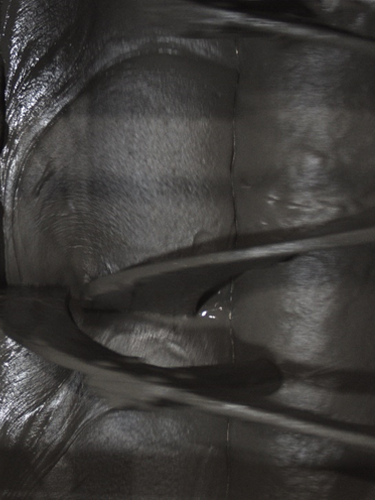
\includegraphics[width=0.24\linewidth]{images/normal.png}}
    \hfill
    \subfloat[Nodular surface]{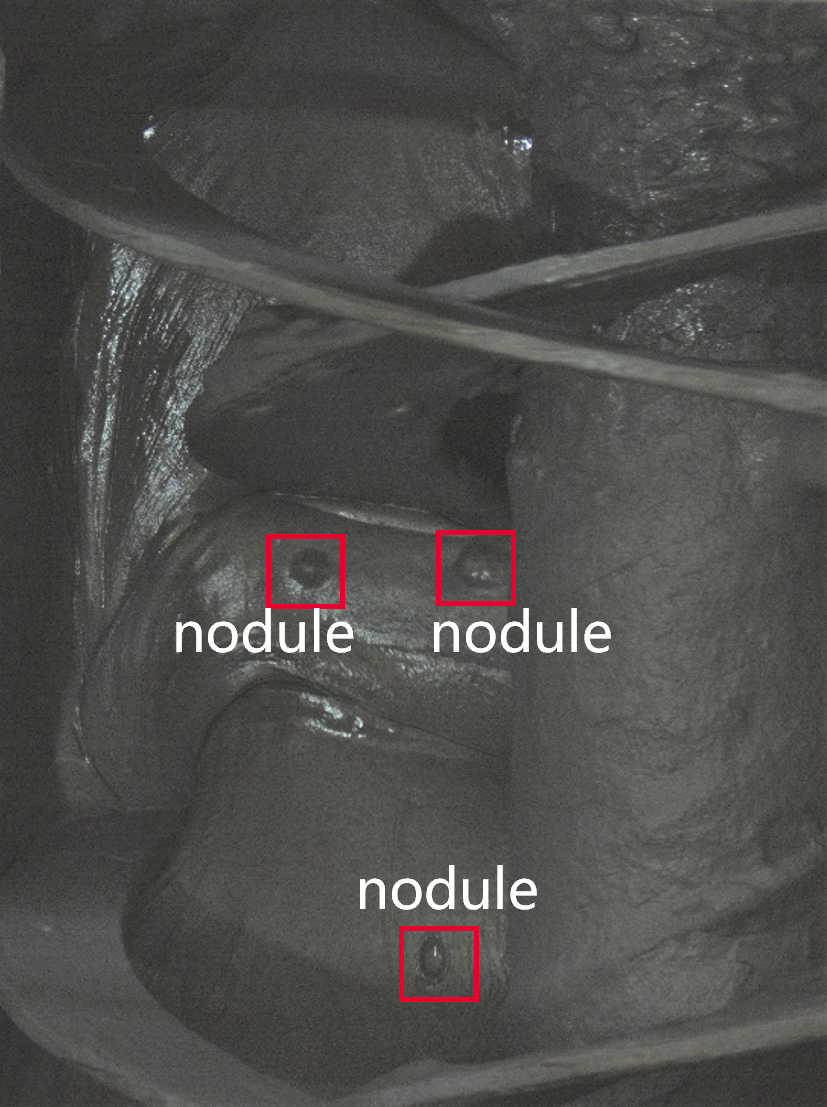
\includegraphics[width=0.24\linewidth]{images/nodular.png}}
    \hfill
    \subfloat[Hump-like surface ]{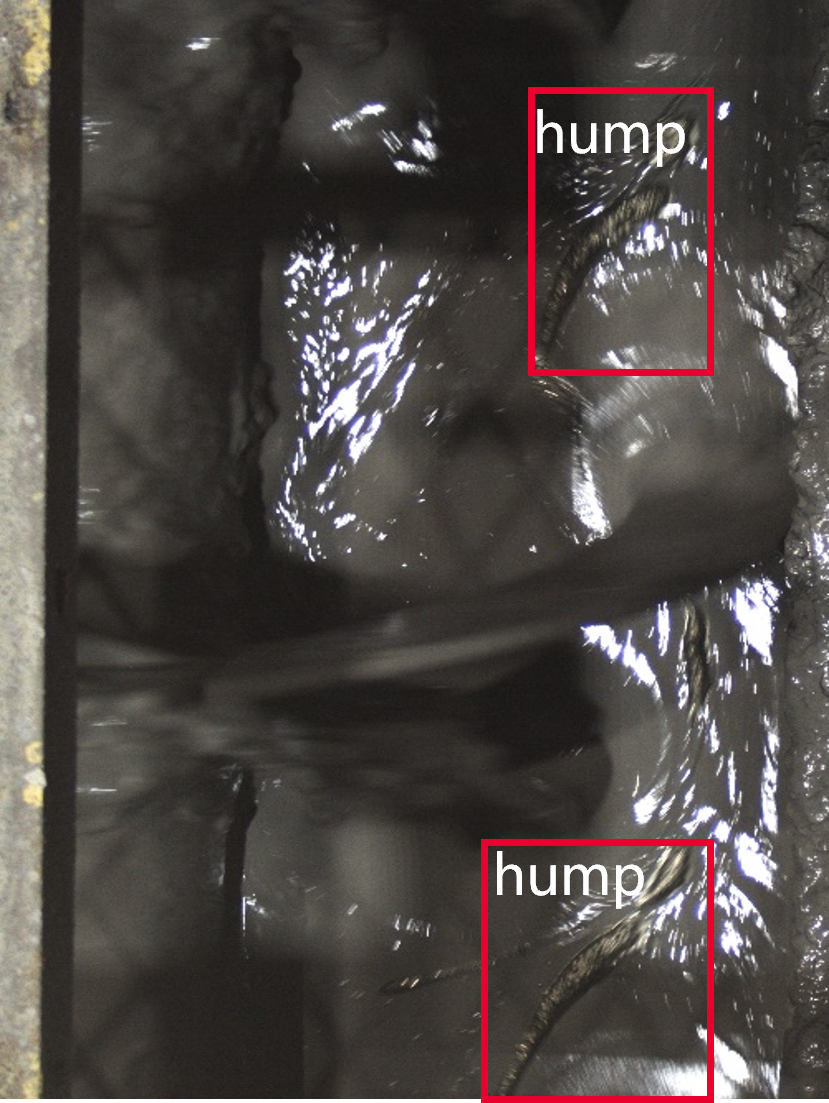
\includegraphics[width=0.24\linewidth]{images/hump.png}}
    \hfill
    \subfloat[Bubble-like surface]{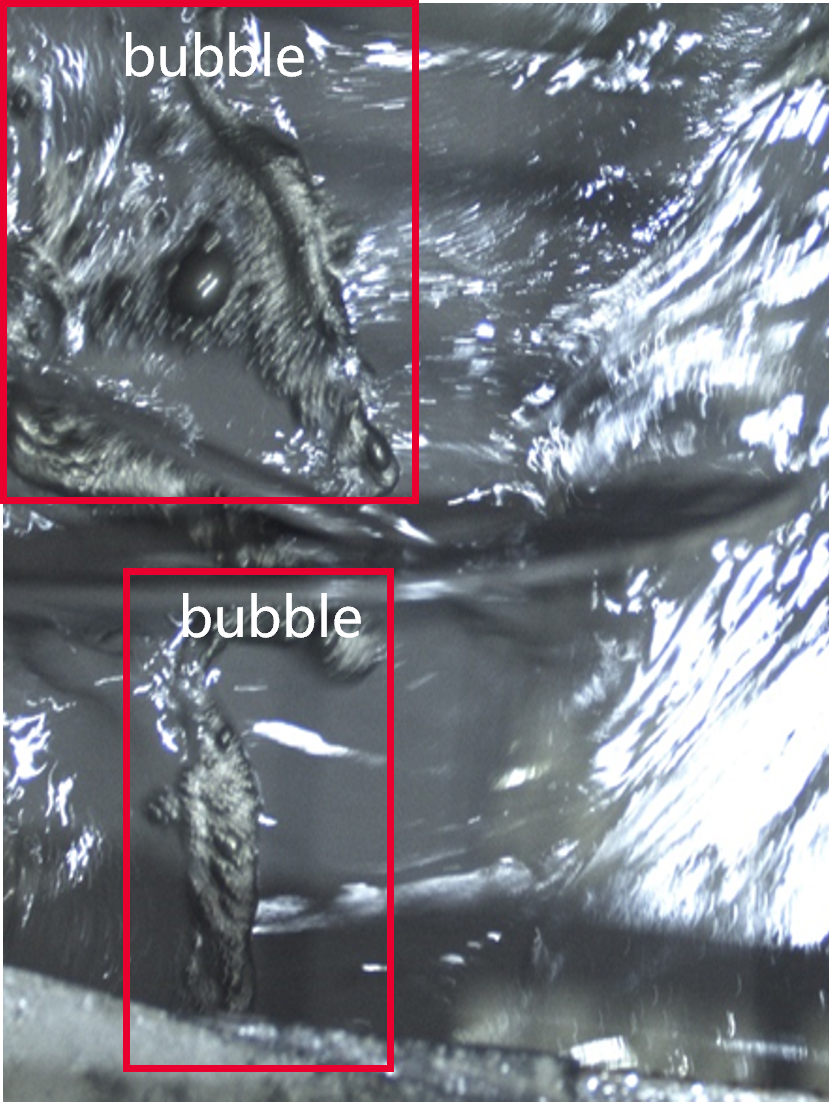
\includegraphics[width=0.24\linewidth]{images/bubble.png}} 
    \caption{surface features of paste}
    \label{fig:surface_features}
\end{figure}


% Many existing studies have measured homogeneity to identify mixing endpoints to improve product quality by computer vision techniques. 
In order to improve the product quality, many existing studies introduce computer vision techniques for measuring homogeneity. 
As an intuitive, low-cost technique, optical image analysis has been widely used in solid-liquid mixing processes\cite{VisionHomoReviewer} such as food\cite{VisionHomoFood}, concrete\cite{VisionHomoInConcrete} and so on. 
However, these studies generally employ color histograms, edge detection to extract features from surface images and only use contrast and grayscale standard deviation as indicators to identify  homogeneity changes.          
These relatively simple image processing techniques can not handle high-level semantic features like lumps and bubbles. 
% With the development of computer vision research, semantic image segmentation algorithms are designed to acquire high level prior knowledge about the semantic meaning of the objects that compose the image\cite{ImageSegmentation}. 

With the development of computer vision research, Deep Convolutional Neural Networks(DCNN) based semantic image segmentation is proposed to partition a digital image into multiple image segments according to the semantic information in nature scene images\cite{ImageSegmentation}.
% According to the output of Deep Convolutional Neural Networks(DCNN), pixels belong to same objects are classified into identical categories.
This technique is widely used in many applications, such as medical image processing and self-driving car.
The high precision and good generalization of deep-learning-based image segmentation inspire us to identify non-paste and non-homogeneous areas in the images.
% We next use the calculate the proportion of non-homogeneous features in paste area. 
%Next, the proportion of non-homogeneous areas in the whole image is employed to quantify the paste homogeneity based on a Gaussian process model by considering the mixer filling factor.
%In order to model the influence of the blade positions on the proportion of non-homogeneous areas, a Gaussian Processes model is fitted to predict the prior distribution of non-homogeneous area under different blade positions.


% In this paper, A state-of-the art image segmentation model deeplab-v3\cite{Chen2017RethinkingAC} were used to identify non-paste and non-homogeneous areas in the images.          
In this paper, we introduce learning-based semantic image segmentation to identify non-paste and non-homogeneous areas in the  images of paste surface.          
We also investigate the performance of different images resolution and preprocessing method with the specific application of non-paste and non-homogeneous task. 
% An empirical model is generated through historical mixing homogeneity data based on Gaussian Process Regression to predict the prior distribution of non-homogeneous area under different blade positions.        
In order to eliminate the effect of blade positions on the evaluated homogeneity, we use the collected paste images and their corresponding non-homogeneous area to fit a Gaussian Process Regression(GPR) model\cite{IJM-12-2021-1162}.
The GPR model is constructed to predict the  distribution of non-homogeneity factor conditioned by different blade positions.

The key contributions are highlighted as follows:
\begin{enumerate}
    \item This paper proposes a computer-vision-based non-contact paste homogeneity measurement pipeline for quantifying and evaluating the paste homogeneity in real-time.
    \item This is the first time the paste homogeneity evaluation is formalized as a semantic image segmentation problem. 
    The self-made dataset, including the images of paste surface and their non-homogeneous area labels, is public released. \footnote{The dataset is available at \url{dataset.ustb-ai3d.cn/paste_homogeneity}}
    
    % We establish and release a paste surface dataset that has non-paste and non-homogeneous area labels, and realized the semantic image segmentation algorithm of the dataset.
    \item The proposed pipeline is deployed and evaluated in a real paste backfill station. 
    The experimental results demonstrate that the technique satisfies the requirements in terms of efficiency, accuracy and stability. The predicted homogeneity metric is intuitively consistent with subjective assessment.
\end{enumerate}
% In this paper, we propose a non-contact and real-time paste homogeneity measurement pipeline to quantify and evaluate the paste homogeneity. We establish and release a paste surface dataset that has non-paste and non-homogeneous area labels, and realized the semantic image segmentation algorithm of the dataset. 
% The experiments conducted in paste backfill station demonstrate that the proposed pipeline satisfies the requirements in terms of efficiency, accuracy and stability, and the homogeneity metric is consistent with subjective assessment.

\section{Methods}\label{sec2}


The proposed pipeline consists of three major steps: data collection, non-homogeneous area identification, and homogeneity quantization. 
First, we collect data with a camera installed above tail of double-shaft mixer. Next, the collected images are fed into an image processing module to identify non-homogeneous areas and non-paste area. 
Then, we defined the non-homogeneity factor as the proportion of the non-homogeneous area to the paste area in an image. 
Finally, we fit a Gaussian Process Regression to predict the prior probability distribution of non-homogeneity factor conditioned by the current blades positions.
The homogeneity metric is determined by the cumulative probability of non-homogeneity factor in the prior distribution.
The pipeline of image collecting and analysis is shown in Fig. \ref{fig:pipeline}. 
% that has occurred historically, to estimate the homogeneity metric.
\begin{figure}[htb]
    \centering
    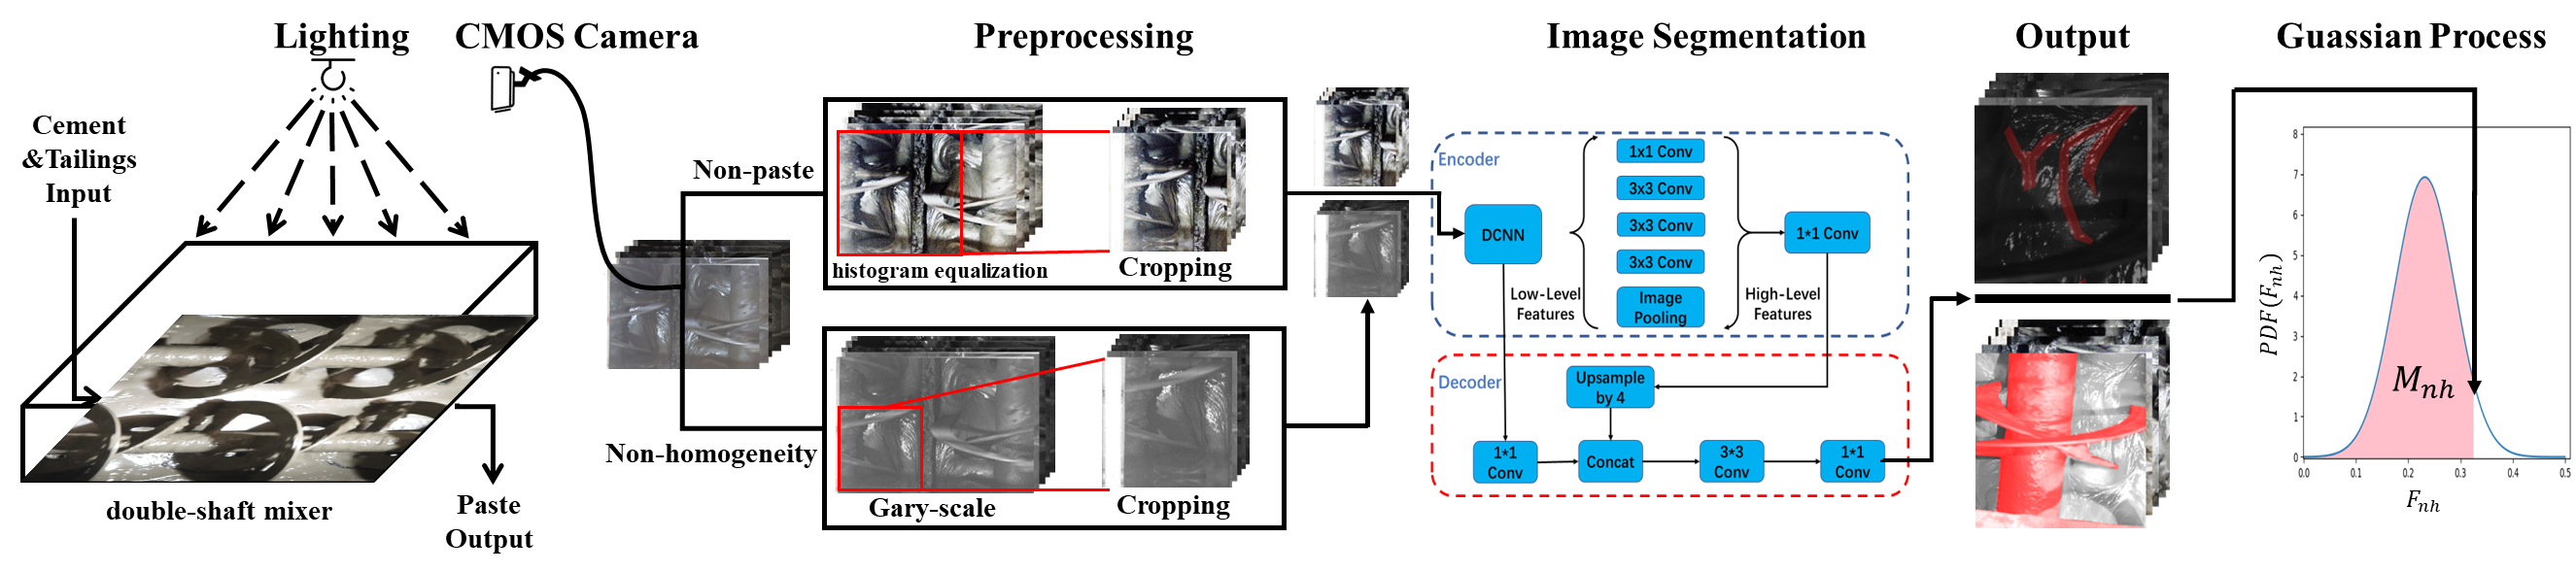
\includegraphics[width=0.99\linewidth]{images/pipeline.png}
    \caption{System overview.}
    \label{fig:pipeline}
\end{figure}

\subsection{Data Collection}

Many previous practices indicate that the main reason leading to the non-homogeneous paste is the agglomeration phenomenon of the particles\cite{wu2019rheology}, 
During the paste mixing, concentrated tailings and cement particles adheres to each other and larger aggregates are formed under the wrapping impact of water film and the adsorption effect of particles\cite{QI2019106025}. 
% The aggregates not only reduce the fluidity of the paste, which increases the risk of pipe vibration and blockage phenomenon, but also reduce to the physical strength of backfill body \cite{tailingsManagement}
Not only the aggregates reduce the fluidity of the paste and increase the risk of pipe vibration and blockage phenomenon, they also reduce the physical strength of backfill body \cite{tailingsManagement}.
Because the shear of the blades plays an important role to avoid the agglomeration phenomenon\cite{yang2019research} in mixer, it is particularly important to identify the paste homogeneity after it passes through the mixer blades. 
The mixing effect between materials is usually completed by diffusion, convection and shear\cite{lacey1954developments}. 
% Diffusion mixing is dominant role for low concentrations of soluble substances, but is limited for the high concentrations of insoluble particles. 
Diffusion mixing plays a major part for the low concentration of soluble substances.
%However, it is limited when the concentration of insoluble particles is high. 
However, it is limited for insoluble particles in tailings and the high concentration of paste.
Convective mixing is effective for the macroscopic mixing, but difficult to break the tiny cement masses and achieve homogenize in micro-structure. 
In comparison to the others, shearing will produce vortex and shear stress fields in which the aggregates will rupture because of stretching and deforming by blades.
% This behavior for achieving microscopic mixing only occurs
% to achieve microscopic mixing of materials, but this action usually occurs only by blades.       

Therefore, we installed a camera at the tail of the double-shaft mixer where the paste would be fully stirred by the blades, as demonstrated in Fig. \ref{fig:pipeline}. 
The collected images will be sent to the server via industrial Ethernet for subsequent process in real-time.


\subsection{Image Preprocessing and Segmentation}

\begin{figure}
    \centering
    \subfloat[Original image.]{\includegraphics[width=0.32\linewidth]{images/original.png}}
    \hfill
    \subfloat[non-paste areas.]{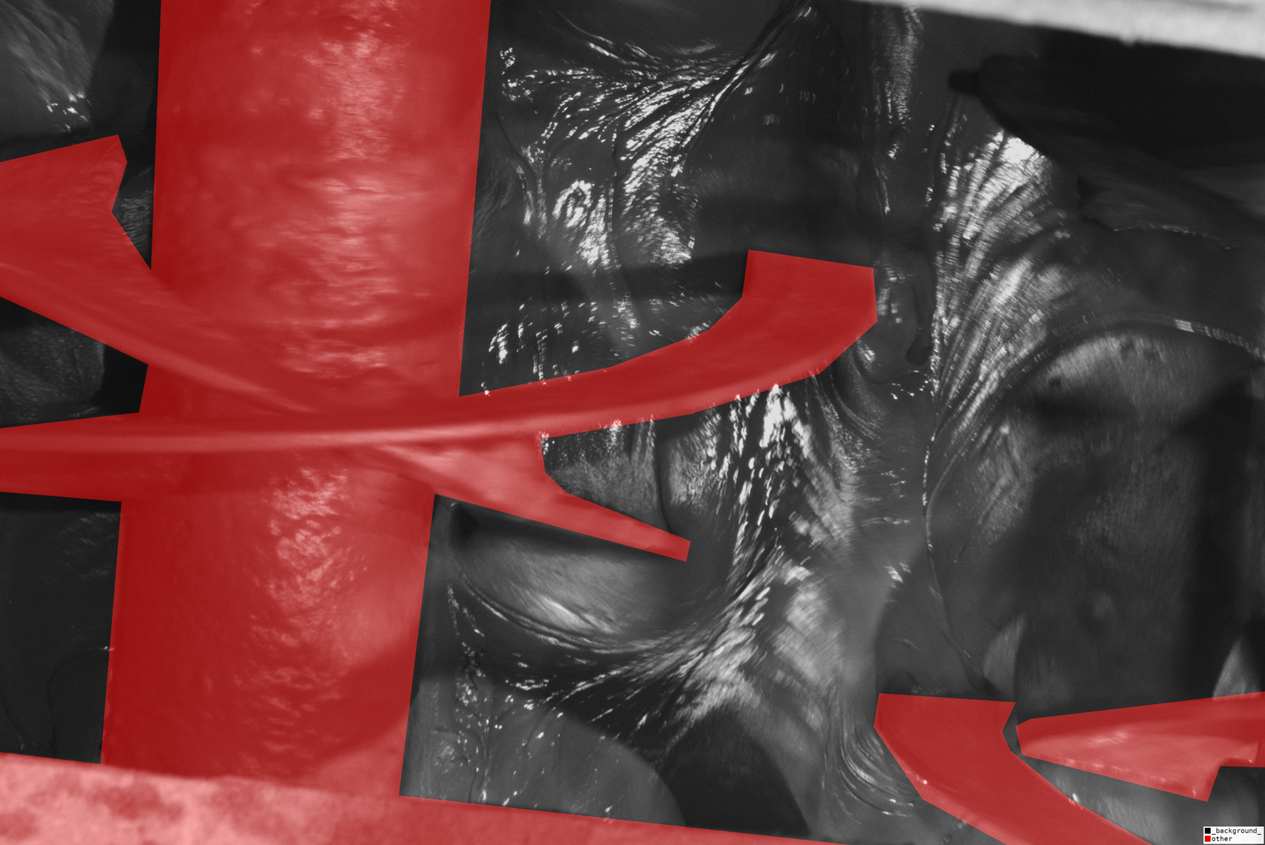
\includegraphics[width=0.32\linewidth]{images/non-paste.png}
    \label{fig:non_paste_demo}}
    \hfill
    \subfloat[non-homogeneous areas.]{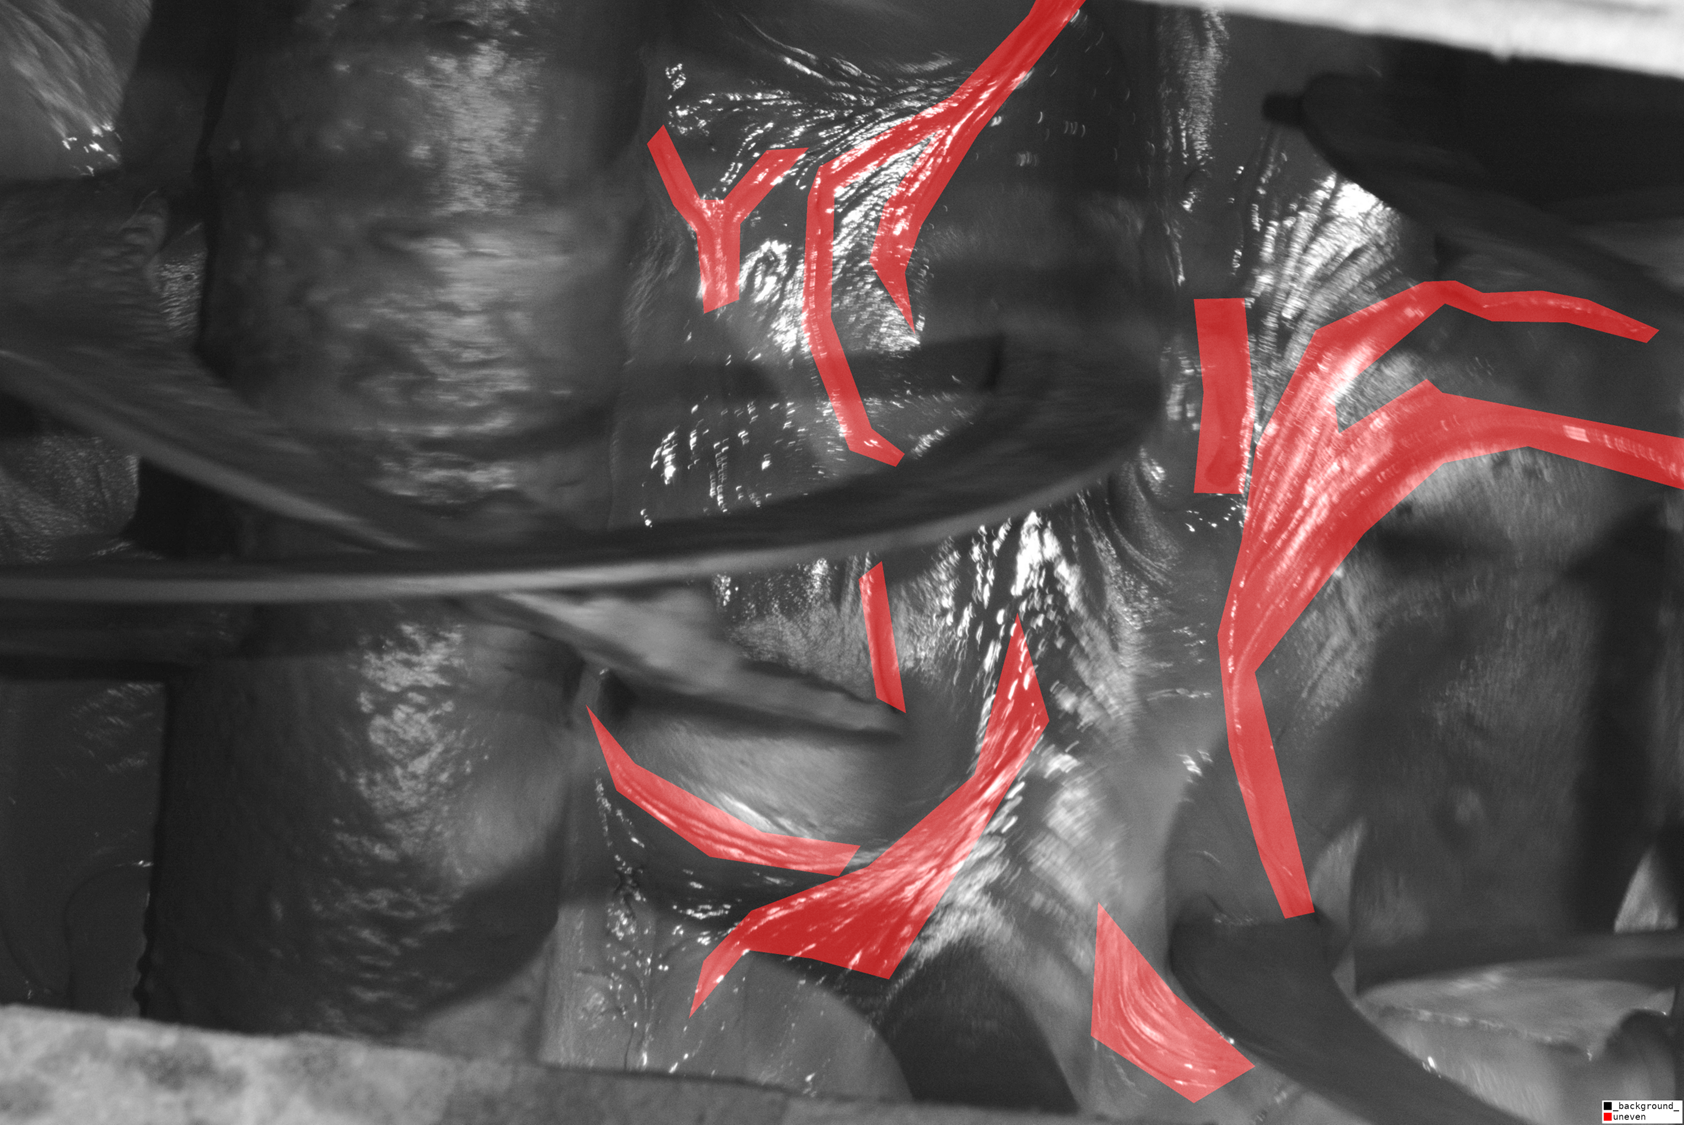
\includegraphics[width=0.32\linewidth]{images/homogenity.png}
    \label{fig:uneven_demo}}
    \caption{Demonstration of segmented areas.}
\end{figure}


In order to determine the homogeneity of an image, we propose to identify areas considered non-homogeneous with an image segmentation model, and determine the non-homogeneity of the image according to the segmentation results. 
Inevitably, not all areas in the captured image are paste area, as shown in Fig. \ref{fig:non_paste_demo}, there are some other objects and areas in the image captured by the CMOS camera, such as the edges of paste containers and blades of mixer. 
In order to ensure such area do not interferes with the results, it is necessary to detect and exclude them before calculating the final metric.      


Therefore this paper uses two independent image segmentation models to identify these non-paste areas and non-homogeneous areas respectively. 
Deeplab-v3, compared with the state-or-the-art methods\cite{swin,ronneberger2015u,Chen2017RethinkingAC}, was chosen as the semantic image segmentation model, because it has stronger multi-scale feature recognition ability.
%and its DCNN module achieve stronger encoding ability for image details. 
%The structure of swin-transformer is too complex, and the operation time is nearly 20 times slower than U-Net and Deeplab-v3, which cannot meet the demand of real-time detection;
\par

\subsubsection{Non-paste area}\label{non-paste-area}
% 这里不能直接讲图片下采样,还缺一段话,为什么要做Non-paste area identification,Non-paste area identification的目的是什么。
Image resolution, brightness, contrast and other image attributes are hyper-parameters of semantic image segmentation model, which will significantly affect the performance of the model.
Although the cameras are able to capture images with high-resolution, it should be noted that the calculating speed and memory usage of CNN are proportional to the resolution of the input image. 
In order to achieve real-time identification,  it is necessary to downscale the resolution of the original image for accelerating the process. But the resolution too small will cause image blurry, we make a trade-off between resizing and cropping through experiments. 
% Ideally, the size of input image should be no more than a few hundred pixels wide and tall in order to meet the real-time requirements. 
In this paper, we first shrink the original images to small resolution of 768x512 and then crop them into several 256×256 sub-images by overlapping tile strategy\cite{ronneberger2015u}.
The cropped images are fed to the segmentation model and the results are stitched back to the result of segmentation with size 768x512.
% the original, down-scaled size.
% , which would be sent into the segmentation model for processing. 
% After processing, the result of the cropped images would be stitched back to the original, down-scaled size. 
Because the non-paste area is large, downscaling the original images is not only beneficial to accelerate, but also prompt the model learn more high-level semantic information from input images.\par
% Furthermore, we conduct histogram equalization on the input images to improve the segmentation result. The purpose of this process is to increase the contrast in the image, thus sharpening the edges and curves in the image to help the model identify the boundaries of the target areas.

Furthermore, 
in order to increase the contrast and sharpen the edges and curves in the image, the histogram equalization method was used aiming at increasing the contrast. 
Experimental results verify that this operation improves the accuracy of identifying boundaries of the non-paste area.
% we conduct histogram equalization on the input images to improve the segmentation result. The purpose of this process is to increase the contrast in the image, thus sharpening the edges and curves in the image to 
% help the model identify the boundaries of the target areas.


\subsubsection{Non-homogeneous area}\label{2.2.2}

% There are many different categories of non-homogeneous features such as humps and bubbles, which varies widely and are distinct from each other. Although it is tempting to distinguish each category from others, this may be difficult because of the data imbalance problem, meaning that some categories have abundant training data, while other categories have only a handful training examples for the model to learn from.
% The occurrence frequency of non-homogeneous features such as humps and bubbles is different, which is referred to as the problem of data imbalance. 
The frequency of non-homogeneous features existing in an image, such as humps and bubbles, is different from each other.
% This means that some categories have abundant training data, while the amount of training examples in other categories  have only a handful  for the model to learn from, which make neural network becomes more difficult to train.
This means that there are abundant training data in some categories, while the amount of training examples in other categories is insufficient for training model, which is also regarded as the problem of data imbalance, which will lead to difficulties in training neural network.

Moreover, different kinds of non-homogeneous features often appear simultaneously and overlap with each other.
It is difficult to accurately label what the categories each pixel belongs to.
Therefore, we assign all pixels in non-homogeneous area into a single category. 
The model is trained to determine whether an area is homogeneous.


Similar to the non-paste area detection in \ref{non-paste-area},
the images captured by camera are resized and cropped before they they are fed into the segmentation model. 
%However, because the non-homogeneous areas are usually smaller than non-paste areas, they contain more small-scaled information which could be lost if the image was downsized too aggressively. 
However, since the size of non-homogeneous features(such as bubble and hump) are usually much smaller than non-paste features(such as the mixing shaft and helmet), aggressive downsizing will make the non-homogeneous features very blurry, which will further increase the learning difficulty of the network.
In order to preserve as much detail as possible, we shrink the original images to 1536×1024 and then crop them to 640×640.
%Though cropping the image into multiple smaller sub-images without resizing it first is an option, empirical results show that such a method does not perform well. We believe this is because the areas in these sub-images only consist of a tiny part of the original image, thus containing too few non-homogeneous areas. The model would have a hard time learning the characteristics of these areas during training. So we chose to resize the input image to a lower resolution of 1536×1024, then cropped to 640×640 size as a trade-off. 
The original color images, meanwhile, are converted to grayscale images for emphasizing the edges.
% so as to obtain the optimal performance of segmentation model.           


\subsection{Quantization of homogeneity}\label{sec2.3}

\subsubsection{non-homogeneity factor}\label{2.3.1}
After identification the non-homogeneous areas and non-paste areas in an image, We believe that the proportion of non-homogeneous area to the paste area reflects the degree of non-homogeneity, so we define the non-homogeneity factor $F_{nh}$ as follows:
\begin{equation}
\label{equ:prop_p}
F_{nh} = \frac{S_{nh}}{{S_{total} - S_{np}}},
\end{equation}
where $F_{nh}\in\left[0,1 \right)$, $S_{nh}$ is the size of identified non-homogeneous areas, $S_{total}$ is the total size of the input image, and $S_{np}$ is the size of non-paste areas.
All variables are measured by pixels.          


\begin{figure}[htb]
    \centering
    \subfloat[image of the blade at position of 68]{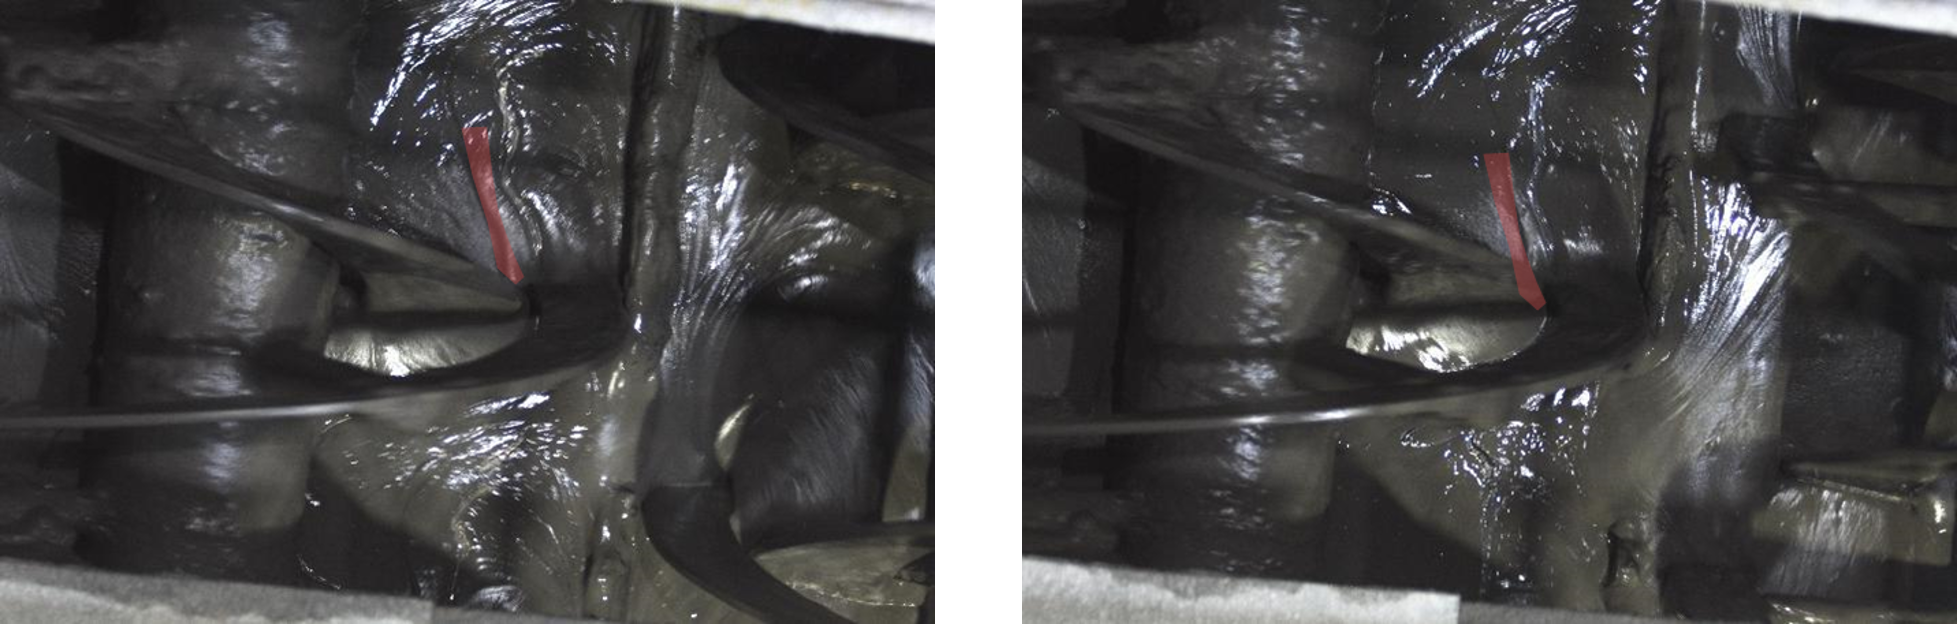
\includegraphics[width=0.48\linewidth]{images/position68.png}}
    \hfill
    \subfloat[image of the blade at position of 115]{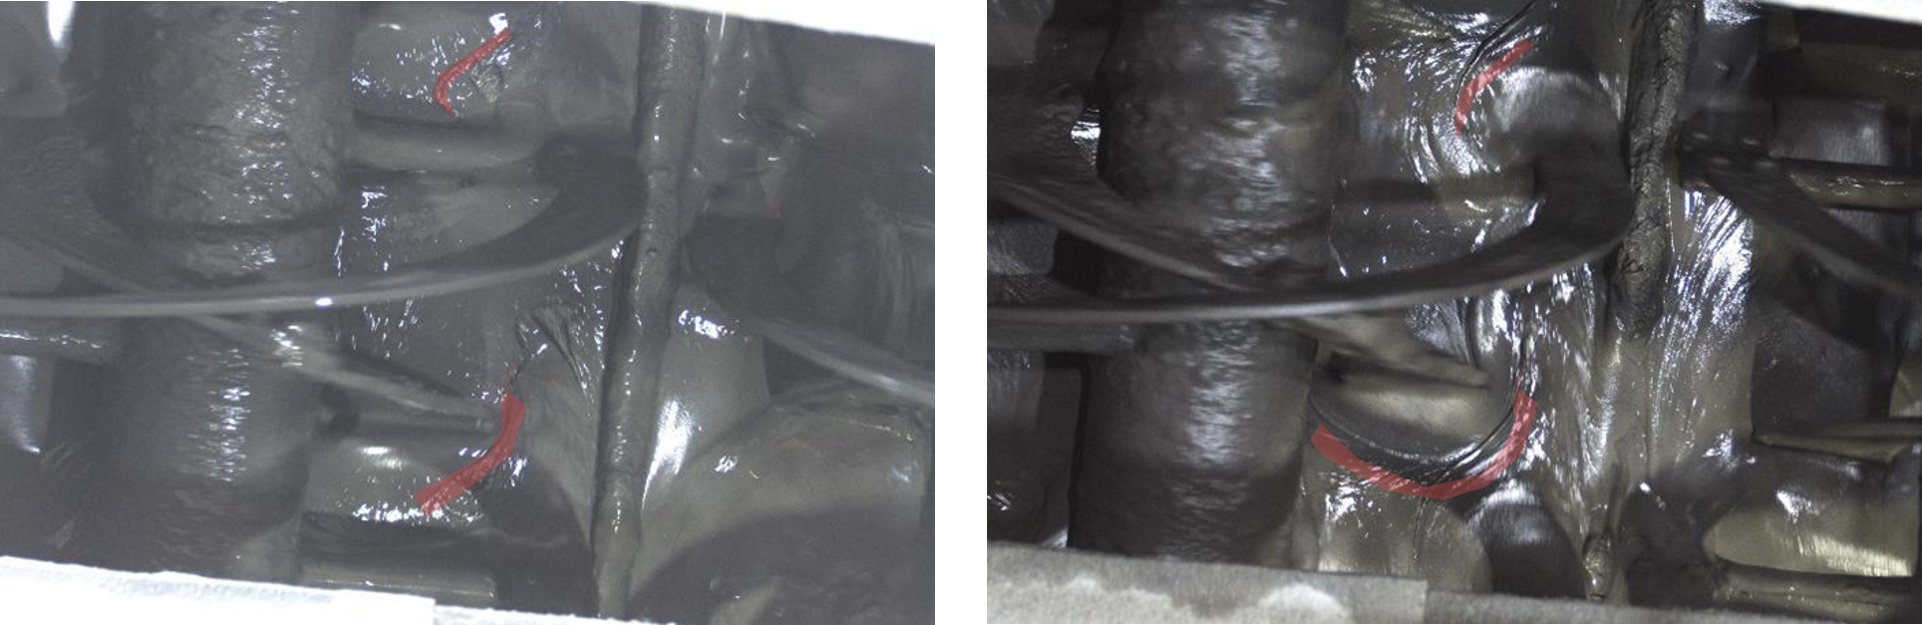
\includegraphics[width=0.48\linewidth]{images/position115.png}}
    \caption{The ripple shape affected by the blade. The images were captured on four different weekdays. The position of blade in each sub-figure a,b is the same. By comparison, it can be seen that the paste morphology is similar under the same blade position, and the morphology is difference under different blade position.}
    \label{ripple comparison}
\end{figure}

Moreover, we discover a correlation between blades positions and non-homogeneity factor. Blades positions will interfere the quantified homogeneity if the empirical value of $F_{nh}$ is assumed to follows a Gaussian distribution. As shown in Fig. \ref{ripple comparison}, the position of blades will affect the paste surface morphology, which leads to different ripple shapes and shadow areas.
For two paste surface images of which the blade position are similar, the non-paste areas and the paste surface flow field are also similar.         


Therefore, this paper introduces Gaussian Process Regression(GPR) to model the relationship between the positions of blades and the prior distribution of homogeneity for evaluating the homogeneity more reliably. 
As a non-parametric regression model, the GPR can be regarded as a generalization of multivariate normal distribution in continuous domain.
When the dataset is small, GPR works better than other prediction models in interpolation tasks\cite{KONG2018556}.

Specifically, the blade position is defined as vertical coordinate $pos_i \in\left[0,200 \right]$ of the top left corner of the blade, which is estimated by comparing the identified non-paste areas with a pre-defined blade template. Training dataset of the GPR is $\mathcal D=\{(pos_i, y_i)\vert i=1,2\,\cdots,N\}$, where $y_i$ is the non-homogeneity factor of the i-th image. GPR can be specified by its mean function $m(x)$ and covariance function $k(x, x’)$:
\begin{equation}
f(\boldsymbol x)\sim\mathcal{GP}(m(\boldsymbol x)\text{,}k(\boldsymbol x\text{,}\boldsymbol x'))
\end{equation}

According to the definition of Gaussian process, the observed values and the function values at new test points follow a joint Gaussian prior distribution which can be represented as:
\begin{equation}
    \begin{bmatrix}y\\f_\ast\end{bmatrix}\sim\mathcal N\left(\begin{array}{c}m(X)\\m(X_\ast)\end{array}\text{,}\begin{bmatrix}K(X\text{,}X)+\sigma_n^2I&K(X\text{,}X_\ast)\\K(X_\ast\text{,}X)&K(X_\ast\text{,}X_\ast)\end{bmatrix}\right)
\end{equation}
where $K$ is the covariance kernel matrix where its entries correspond to the covariance function evaluated at observations, $X$ is the training dataset,  $X_*$ is the test dataset, $\sigma_n$ is the standard deviation of the noise. Matern kernel is used to fit the function between the blade position and the distribution of homogeneity proportion. The Matern kernel are defined as follows:
\begin{equation}
   k_{\text{Matern}}(\mathbf{x}, \mathbf{x'}) = \frac{2^{1 - \nu}}{\Gamma(\nu)}
   \left( \sqrt{2 \nu} d \right)^{\nu} K_\nu \left( \sqrt{2 \nu} d \right)
\end{equation}
where $d = (\mathbf{x} - \mathbf{x'})^\top \Theta^{-2} (\mathbf{x} - \mathbf{x'})$ is the distance between $x$ and $x'$ scaled, $\Theta$ is a length scale parameter, $\nu$ is a smoothness parameter, the smaller the less smooth, $K_\nu$ is a modified Bessel function, $\Gamma$ is the gamma function. 
Given the training data set and test points, a posterior distribution on $f_*\sim\mathcal N(\bar{f}_{*},cov(f_{*}))$ can be derived, where
\begin{equation}
\small
\bar{f}_{*}=\mathbb{E}\left[f_{*} \mid X, \boldsymbol{y}, \boldsymbol{x}_{*}\right]=m\left(X_{*}\right)+K\left(X_{*}, X\right)\left[K(X, X)+\sigma_{n}^{2} I\right]^{-1}(\boldsymbol{y}-m(X))
\end{equation}
\begin{equation}
\operatorname{cov}\left(f_{*}\right)=K\left(X_{*}, X_{*}\right)-K\left(X_{*}, X\right)\left[K(X, X)+\sigma_{n}^{2} I\right]^{-1} K\left(X, X_{*}\right)
\end{equation}

$\overline{f_*}$  is the predicted output of the GPR model for test point. Confidence interval (CI) of the predicted output value can be determined by the variance $cov(f_*)$.
% $\Theta$ is the identity matrix, $\nu$ is taken as 2.5.
\par
% Specifically, the position of blade can be measured by comparing a pre-defined blade template with the non-paste areas identified in the previous steps. 
% We find the position of the top left corner of the blade, then use the y-coordinate of the position as the independent variable of the Gaussian process because the x-coordinate of the blade is always on the rotation shaft. 

For any blade position, the GPR can predict a corresponding Gaussian distribution for determining whether the non-homogeneity factor is within normal limits.\par



\subsubsection{Homogeneity metric}\label{2.3.2}

 After fitting the historical non-homogeneity factor distribution with GPR, it is easy to calculate the probability that the history is more homogeneous than a new non-homogeneous factor.       
 
Thus the homogeneity metric $M(F_{nh}) \in [0,1]$ is defined by the cumulative distribution function(CDF) of the random variable non-homogeneity factor $F_{nh}$ to judge the degree of paste homogeneity,  which can be denoted as:
\begin{equation}
    M(F_{nh}) =1- P(F_{nh} \leq f_{nh})=\int_{0}^{f_{nh}}\frac{1}{\sqrt{2 \pi} cov(f_*)} \exp \left(-\frac{(x-\bar{f_*} )^{2}}{2  cov(f_*)^{2}}\right)
\end{equation}
where $f_*$ is the posterior Gaussian distribution  corresponding to the GPR fitted according to blade position, $f_{nh}$ is the non-homogeneity factor calculated according from the image.

\section{Experiments}\label{sec5}
The following section will examine the proposed pipeline from three perspectives: 
non-paste area identification, non-homogeneous area identification, and the necessity of introducing the GPR.\par
The image used in training segmentation models were all collected in the production environment of a real copper mine. In the total available images, 1033 images were used as the dataset for the non-paste area identification task, and 220 were used as the dataset for the non-homogeneous area identification task. 
All images were manually labelled in advance. 
Each dataset was randomly divided into training set, validation set and test set with a ratio of 3:1:1.         

The models are implemented based on PyTorch framework. 
We use the unified focal loss \cite{YEUNG2022102026} as loss function for training and the learning rate is set to 2e-5. 
The unified focal loss is a compound loss function that unifies Dice-based and cross entropy-based loss functions to better handle class imbalanced problems\cite{MA2022204}. 
Since our task is a class imbalanced segmentation problem, meaning that the sizes of foreground and background elements are highly unequal, the unified focal loss is suitable for our problem. 
The model for identification non-paste area is trained for 75 epochs, while the model for detecting non-homogeneous area is trained for 250 epochs due to the increased difficulty of the task. 
Our system is deployed on a server with a single Nvidia 1080Ti GPU, which can meet the demand of real-time identification in the industrial field.         


The pixel accuracy and dice coefficient are chosen for evaluating the performance of two segmentation tasks. 
Pixel accuracy is one of the most commonly used evaluation metrics in the field of image segmentation, which is defined as$ \frac{\left\|  P\cap G \right\| + \left\| \neg P\cap \neg G \right\| }{\left\| P+\neg P \right\| }$, where G indicates ground truth areas, P indicates the predicted areas,$\neg P$ is the area outside the predicted area in the picture, and $\left\|G\right\|$ and is the number of pixels in the ground truth area\cite{long2015fully}. 
In contrast to the pixel accuracy, Dice coefficient focuses on gauging the similarity of predicted areas and truth areas, which is defined as $\frac{2\left\|P\cap G\right\|}{\left\|P\right\| + \left\|G\right\|}$.
Dice coefficient pays more attention to the correctly segmented foreground areas, which is more suitable for class imbalance segmentation problem where the foreground area is small.



\subsection{Input Resolution}

\begin{table}[]
\caption{Comparison between different input resolution}
\label{InputResolution}
\resizebox{\columnwidth}{!}{%
\begin{tabular}{@{}ccccc@{}}
\toprule
\multirow{2}{*}{Input resolution} & \multicolumn{2}{c}{Non-paste identification} & \multicolumn{2}{c}{Non-homogeneity identification} \\ \cmidrule(l){2-5} 
                                  & Accuracy             & Dice coefficient      & Accuracy                & Dice coefficient         \\ \midrule
5496×3672                         & -                    & -                     & 0.9282                  & 0.5025                   \\
2304×1536                         & -                    & -                     & 0.9446                  & 0.4998                   \\
1536×1024                         & 0.9011               & 0.8873                & \textbf{0.9459}         & \textbf{0.5855}          \\
768×512                           & 0.9349               & \textbf{0.9279}       & 0.9443                  & 0.5718                   \\
384×256                           & \textbf{0.9365}      & 0.9264                & -                       & -                        \\ \bottomrule
\end{tabular}%
}
\end{table}


The resolution of original captured images is  5496×3672, which is roughly 3:2. 
Therefore, we choose to maintain the 3:2 width to height rate for all resolutions of input images.\par
The results for different input resolutions are shown in Table \ref{InputResolution}. 
In both tasks, properly reducing input resolution has a drastic positive impact on segmentation accuracy. For non-homogeneous task, the accuracy raised by roughly 2 percent and the dice coefficient by 8 percent by means of lowering the resolution. Of course, using input images with too low a resolution will lead to degraded model performance, since the details of the pasted surface are lost. We observed similar performance improvements for non-paste area identification tasks.\par
It should be noted that the results of non-paste area identification will need to be combined with non-homogeneity areas for further calculation, and to generate a video stream of visualized results for manual reference. Using a resolution too small will cause a huge loss of fidelity, thus affecting the accuracy of homogeneity metric calculation and artificial inspection. \par


\subsection{Image Preprocessing}


\begin{table}[]
\caption{Comparison between different preprocess methods}\label{tabe}
\resizebox{\columnwidth}{!}{%
\begin{tabular}{@{}ccccc@{}}
\toprule
\multirow{2}{*}{Preprocess method} & \multicolumn{2}{c}{Non-paste identification} & \multicolumn{2}{c}{Non-homogeneity identification} \\ \cmidrule(l){2-5} 
                                   & Accuracy          & Dice coefficient         & Accuracy             & Dice coefficient            \\ \midrule
None                               & 0.9311            & 0.9213                   & 0.9503               & 0.6560                      \\
Histogram equalization                 & \textbf{0.9365}            & \textbf{0.9264}                   & \textbf{0.9596}               & 0.6585                      \\
Greyscale                          & 0.9326            & 0.9241                   & 0.9590               & \textbf{0.7017}                      \\
Greyscale and Histogram equalization   & 0.9321            & 0.9225                   & 0.9471               & 0.5985                      \\ \bottomrule
\end{tabular}%
}
\label{Preprocess}
\end{table}

The results for using different preprocess methods are shown in Table \ref{Preprocess}. For non-paste identification task, conducting histogram equalization on input images would give the greatest boost to the performance of the model. For non-homogeneity identification task, converting the image to greyscale gives the biggest boost to model performance. The results also show that it is important to choose proper preprocessing method for each specific task instead of using a single preprocessing method over all tasks.

\subsection{Gaussian Process Prediction model}
\begin{figure}
    \centering
    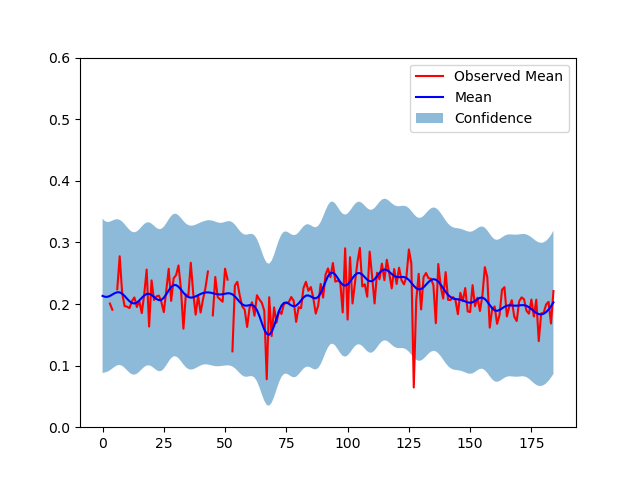
\includegraphics[width=0.99\linewidth]{images/GP_result.png}
    \caption{GPR model fitting results}
    \label{fig:gpr}
\end{figure}

The experimental results of the Gaussian process model shown in Fig. \ref{fig:gpr} further reveal that the non-homogeneous area is indeed related to the blade position. The inner and outer blades move in opposite directions, and we observe that when the two paddles intersect in the middle of the picture (position 60-80 on Fig. \ref{fig:gpr} x-axis), the non-homogeneous area in the paste surface decreases significantly. 
When the two blades gradually separate and approach the next blade, the non-homogeneous area shows periodic fluctuations that first increase and then decrease.


\subsection{Result Analysis}
\begin{figure}
    \centering
    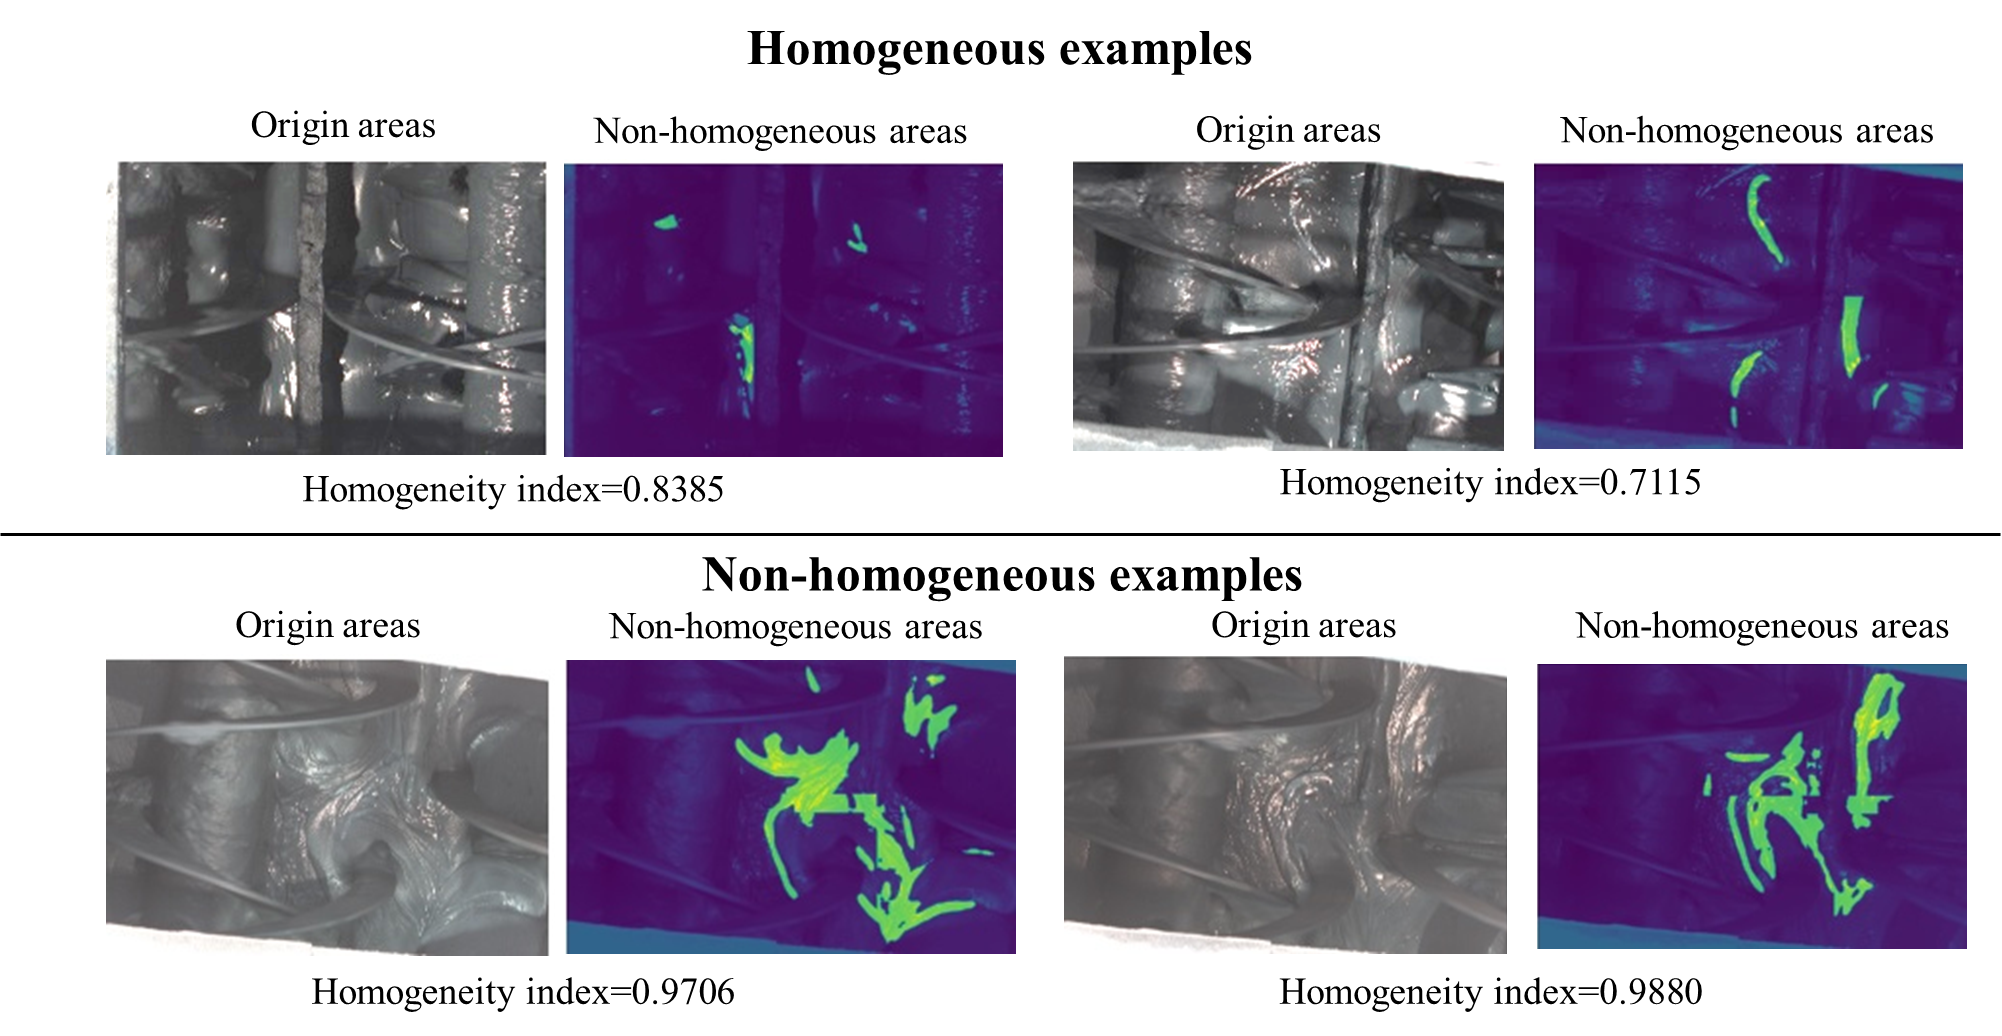
\includegraphics[width=0.98\linewidth]{images/qualitative_demonstration.PNG}
    \caption{Qualitative comparison.}
    \label{fig:qualitative_comparison}
\end{figure}

In Fig. \ref{fig:qualitative_comparison}, we illustrate the comparison of the original image with the result predicted by our model . 
Obviously, when the paste surface is flat and smooth with few hump and nodule cases, the model barely identifies the non-homogeneous areas and thus gives a high homogeneity metric. 
When the paste surface is rougher and filled with more irregular textures, the model can identify large non-homogeneous areas.
If the measured non-homogeneous metric is higher than a specific threshold, the system will alert the engineers to the situation of poor homogeneity and remind the operators to raise the mixing speed or extend the mixing time.
% The visual effect and low homogeneity metric to alert the field engineers.

\section{Conclusion}\label{sec6}

(1) Paste homogeneity is an important evaluation criterion for mixing quality. In this paper, we propose the image segmentation network model to quantify the proportion of non-homogeneous area in the paste area. The appropriate preprocessing method and input resolution were selected by comparing different experimental results to make the segmentation model achieve optimal results, and the accuracy of the model is 93.49\% for non-paste task and 94.59\% for non-homogeneous task.     

(2) We calculate the degree of deviation of non-homogeneity factor from historical data by GPR model to realize a real-time online detection algorithm for paste homogeneity. The experiments of the GPR model demonstrate that the blade position affects the surface morphology of the paste, and images with the same blade position should be used to evaluate the non-homogeneity degree of each other.        

(3) The experiments prove that our designed homogeneity metric results are similar to engineers' subjective assessment and can be used as a quantitative analysis metric to measure the paste non-homogeneity.


\bibliography{sn-bibliography}% common bib file
%% if required, the content of .bbl file can be included here once bbl is generated
%%\input sn-article.bbl

%% Default %%
%%\input sn-sample-bib.tex%

\end{document}
